\section{Methods of signal reconstruction}
\label{sec:signal}


Unlike the resistance of bolometers that can be directly measured to return a signal proportionnal to the incident power, the monitoring of the evolution of the resistance of a KID requires a more complex readout scheme. In fact, one of the challenges of operating a KID is to convert the \I(t) and \Q(t) values to an absorbed optical power or shift in resonant frequency as a function of time $\delta f_{0} \propto \delta P_{opt}$. In this
section, we will see how to adress this problem by using a new modulated readout technique and then by using two different signal reconstruction methods : \rf and \cf.

\subsection{Modulated readout technique}
An innovative readout technique has been developed to monitor the change of the signal by using a known frequency shift. This scheme allows a continuous and simultaneous tracking of KID resonant frequency that changes proportionally to the absorbed optical power. To do so, the standard excitation of the detectors with a fixed tone is replaced by a new excitation based on two different frequencies. In fact, in order to generate two tones, we modulate the local oscillator signal between two values, separated by $\delta f_{LO} \simeq 1$ kHz, and obtain $f_{+} = f_{0} + \frac{\delta f_{LO}}{2}$ and $f_{-} = f_{0} - \frac{\delta f_{LO}}{2}$ with $f_{0}$ the detector resonant frequency.\\
The values ($I(t)$,$Q(t)$) are then given by :

\begin{equation}
(I(t),Q(t)) = (\frac{I(f_{+}) + I(f_{-})}{2}, \frac{Q(f_{+}) + Q(f_{-})}{2}),
\end{equation}

and the differential values are :

\begin{equation}
\label{gradient}
(\delta I(t), \delta Q(t)) = (\frac{I(f_{+}) - I(f_{-})}{\delta f_{LO}}, \frac{Q(f_{+}) - Q(f_{-})}{\delta f_{LO}}).
\end{equation}

\begin{figure}[h]
\center
	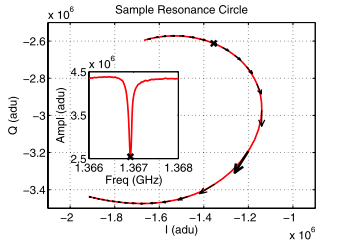
\includegraphics[scale=0.8]{Figures/resonance-circle.png}
	\caption{Representation in the I-Q plane of a sweep around a resonance. The red line represents the $(I,Q)$ data of the frequency sweep around the resonance.The arrows represent ($\delta I$,$\delta Q$). \citep{2013A&A...551L..12C}}
	\label{circle-iq}
\end{figure}

Fig. \ref{circle-iq} shows a typical KID resonance circle. Thanks to this
modulation technique, we obtain four quantities : \I, \Q and their variation
$\delta I$, $\delta Q$.\\ In this paper, \I(t) and \Q(t) are sampled at 22 Hz,
they are the mean values of sub-sample $i$(t) and $q$(t) on $N_{m}$ = 40 points at
880 Hz. \di(t) and \dq(t) are the mean values of the difference between the data
measured at $f_{-}$ and $f_{+}$. Then we have :

\begin{eqnarray}
I  &=& \sum^{N_{m}=40}_{p=1} i_{p},\\
%\label{eq:i}
Q  &=& \sum^{N_{m}=40}_{p=1} q_{p},\\
%\label{eq:q}
dI &=& \sum^{N_{m}/2=20}_{p=1} i_{2p} - i_{2p-1},\\
dQ &=& \sum^{N_{m}/2=20}_{p=1} q_{2p} - q_{2p-1},
\end{eqnarray}

% on voit les equations \ref{eq:i}, \ref{eq:q}.\\

With these quantities in hands we have several ways to derive the transmitted signal. They are presented in the following paragraph.

\subsection{RfdIdQ}
If a variation $\Delta I(t)$, $\Delta Q(t)$ is observed between successive  ($I(t)$, $Q(t)$) points, it is possible to estimate the shift of the resonant frequency $\Delta f_{0}$ between two samples by comparing ($\Delta I(t)$, $\Delta Q(t)$) with the gradient $(\delta I(t), \delta Q(t)) $. This is done by projecting ($\Delta I(t)$, $\Delta Q(t)$) along the gradient found in Eq.\ref{gradient}. $\Delta f_{0}$ is then determined by integrating Eq.\ref{eq:Rf} \citep{2014A&A...569A...9C}.

\begin{equation}
\label{eq:Rf}
\Delta f_{0} = \delta f_{LO} \frac{\Delta I < I >_{50} + \Delta Q < Q >_{50}}{< I >_{50}^{2} + < Q >_{50}^{2}}
\end{equation}

%\delta f_{LO} \frac{\Delta I <dI>_{50} + \Delta Q <dQ>_{50}}{<dI>_{50}^{2} + <dQ>_{50}^{2}}

where $<.>_{50}$ means that we average the considered quantities over 50 points before and after the concerned value, and $\delta f_{LO} \simeq 1$ kHz.

This method is convenient, but can be affected by some systematic uncertainty and be a source of non-linearity. In fact, $(\delta I(t), \delta Q(t))$ is tangent to the (\I,\Q) circle for a fixed background optical power, whereas the actual variation ($\Delta I$, $\Delta Q$) occurs for a fixed excitation frequency and is due to a difference in the optical power, that includes a change in the (\I,\Q) circle radius. As a consequence, the observed (\I,\Q) trajectory is not precisely parallel to the direction given by $(\delta I(t), \delta Q(t))$. The predicted error induced by the projection method is less than 2\% for faint sources \citep{2013A&A...551L..12C}. In addition, by averaging $dI$ and $dQ$ we apply a $dI$, $dQ$ that can be very different from reality, in particular when we are near the resonance, with a bright source.\\

\subsection{Circle fit : Cf}
To compensate for the errors brought by the \rf method, we developed a new technique named \cf.\\
The idea of this method is to project \I,\Q, \di, \dq, onto an axis $y_{3}$ which is as linear as possible with frequency, and so is assumed to be linear with the optical power. In fact, we suppose that :

\begin{equation}
\label{hyp-f}
f = f_{0} + \frac{w}{2} \tan \frac{\phi}{2}.
\end{equation}

We know that near a resonance $Z = I+jQ$ is on a circle. To construct $y_{3}$ we scale, translate, rotate and inverse the initial circle to transform it into an infinite radius circle described by :

\begin{equation}
\label{Zres}
Z_{res} = 1 - j \tan \frac{\varphi}{2}.
\end{equation}

According to Eq. \ref{hyp-f}, the imaginary part of $Z_{res}$ is linearly dependent to the frequency and so represents $y_{3} \propto f - f_{0}$.\\
Here to calibrate this dependency and reconstruct the signal, we use \I, \Q, \di and \dq measurements. By applying the transformations, \I, \Q, \di and \dq become : 

\begin{eqnarray}
I_{res} &=& \frac{1}{2r}[(I-x_{c}) \cos \alpha + (Q - y_{c}) \sin \alpha] + \frac{1}{2}, \\
Q_{res} &=& \frac{1}{2r}[-(I-x_{c}) \sin \alpha + (Q - y_{c}) \cos \alpha], \\
dI_{res} &=& -\frac{1}{2r}(dI \cos \alpha + dQ \sin \alpha), \\
dQ_{res} &=& \frac{1}{2r}(-dI \sin \alpha + dQ \cos \alpha),
\end{eqnarray}

with : ($x_{c}, y_{c}$), r and $\alpha$ respectively, the center, radius and rotation angle of the initial circle.\\
Then, $dy_{3} = Im(dZ_{res})$. According to the hypothesis in Eq. \ref{hyp-f}, $f$ is a polynom, so to reconstruct the shift of the resonant frequency we can easily fit $\frac{\Delta f}{dy_{3}}$ by a polynomial function and integrate it to obtain the relative frequency of the KID.\\

With the modulated readout technique we can calculate \I, \Q, \di, \dq, and use these two methods to monitor the shift of the resonant frequency and derive the corresponding incident power. In the following section, in the interest of KIDs spatialization we will use these methods to study KIDs specific systematics effects by simulating their response to different sources.